\section{Reasoning}
\label{sec-reasoning}

In this section, we briefly introduce the construction of inference graph to infer the hidden attributes.  
The inference graph is constructed using Bayesian network described by a pair $\mathfrak{B}=<\mathcal{G},\mathit{\Theta}_\mathcal{G}>$. 
Specifically, the notation $\mathcal{G}$ is a directed acyclic graph, of which the $i$-th vertex corresponds to a random variable $X_i$, and the connected edge in $\mathcal{G}$ between two vertexes indicates the dependency. 
The second item $\mathit{\Theta}_\mathcal{G}$ is a set of parameters used to quantify the dependencies of $\mathcal{G}$.
We use the notation $\theta_{X_i | \text{Pa}(X_i)} = P_\mathfrak{B}(X_i| \text{Pa}{(X_i)})$ to denote the parameter of $X_i$, of which $\text{Pa}(X_i)$ is the attributes of the parents of $X_i$.
The joint probability distribution of Bayesian network is given by:

\begin{equation}\label{eq:BNOri}
P_\mathfrak{B}(X_1, \cdots, X_n) = 
\prod_{i=1}^{n} P_\mathfrak{B}(X_i| \text{Pa}{(X_i)})=
\prod_{i=1}^{n} \theta_{X_i | \text{Pa}(X_i)}
%\theta_{x_1|\text{Pa}_1(\mathbf{x})}\theta_{x_2|\text{Pa}_2(\mathbf{x})}\cdots \theta_{x_n|\text{Pa}_n(\mathbf{x})}
\end{equation}
\vspace{-1ex}

In our inference graph, the role of Bayesian network is to predict the object class when given the attributes $\{X_i\}_{i=1}^n$ as input. In the sense of probability, the object class is also a variable.
Let $Y=X_0$  be the class variable, the network now has one extra vertex $Y$.
According to the Bayesian rule, the network can be rewritten as:

\vspace{-1ex}
\begin{align}\label{eq:BNWithCls}
\begin{split}
P_\mathfrak{B}(Y|{X}) & = 
\frac{ P_\mathfrak{B}(Y) P_\mathfrak{B}({X}|Y) }{P_\mathfrak{B}({X})}\\
&=\frac{ \theta_{Y|\text{Pa}({X}_0)} \prod_{i=1}^{n} \theta_{X_i|Y, \text{Pa}({X}_i)} }{ \sum_{y'\in \mathcal{Y}} \theta_{y'|\text{Pa}({X}_0)} \prod_{i=1}^{n} \theta_{X_i|y', \text{Pa}({X}_i)} }
\end{split}
\end{align}
where $\mathcal{Y}$ is the set of classes.

%\begin{figure}[tb]
%\centering
%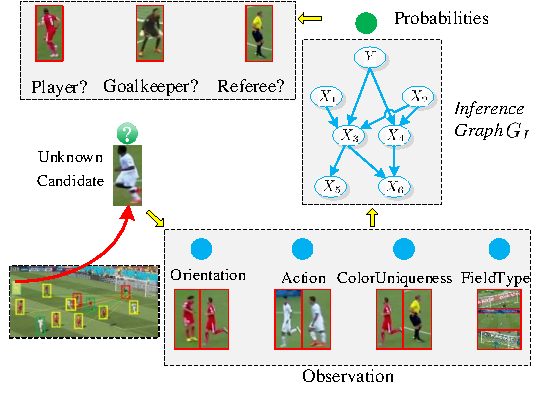
\includegraphics[width=\columnwidth]{inferGraphWorkflow}
%\caption{The pipeline of inference graph used for inferring the role of a person object.}
%\vspace{-4ex}
%\label{fig:inferGraphWorkflow}
%\end{figure}

In the context of Na\"{i}ve Bayes, 
the importance of $P_\mathfrak{B}(Y|{X})$ is stressed by taking the class variable as the root, and all attributes are conditionally independent when taking the class as a condition. As a consequence, the calculation can be simplified as:

\begin{equation}\label{eq:BN-naiveBayes}
P_\mathfrak{B}(Y| {X}) = c \cdot \theta_Y \prod_{i=1}^{n}\theta_{X_i|Y}
\end{equation}
where $c$ is used to make the calculation being a distribution: $c=\sum_{y'\in \mathcal{Y}}  \theta_{y'} \prod_{i=1}^{n}\theta_{X_i|y'}$.

%\begin{figure}[tb!]
%\centering
%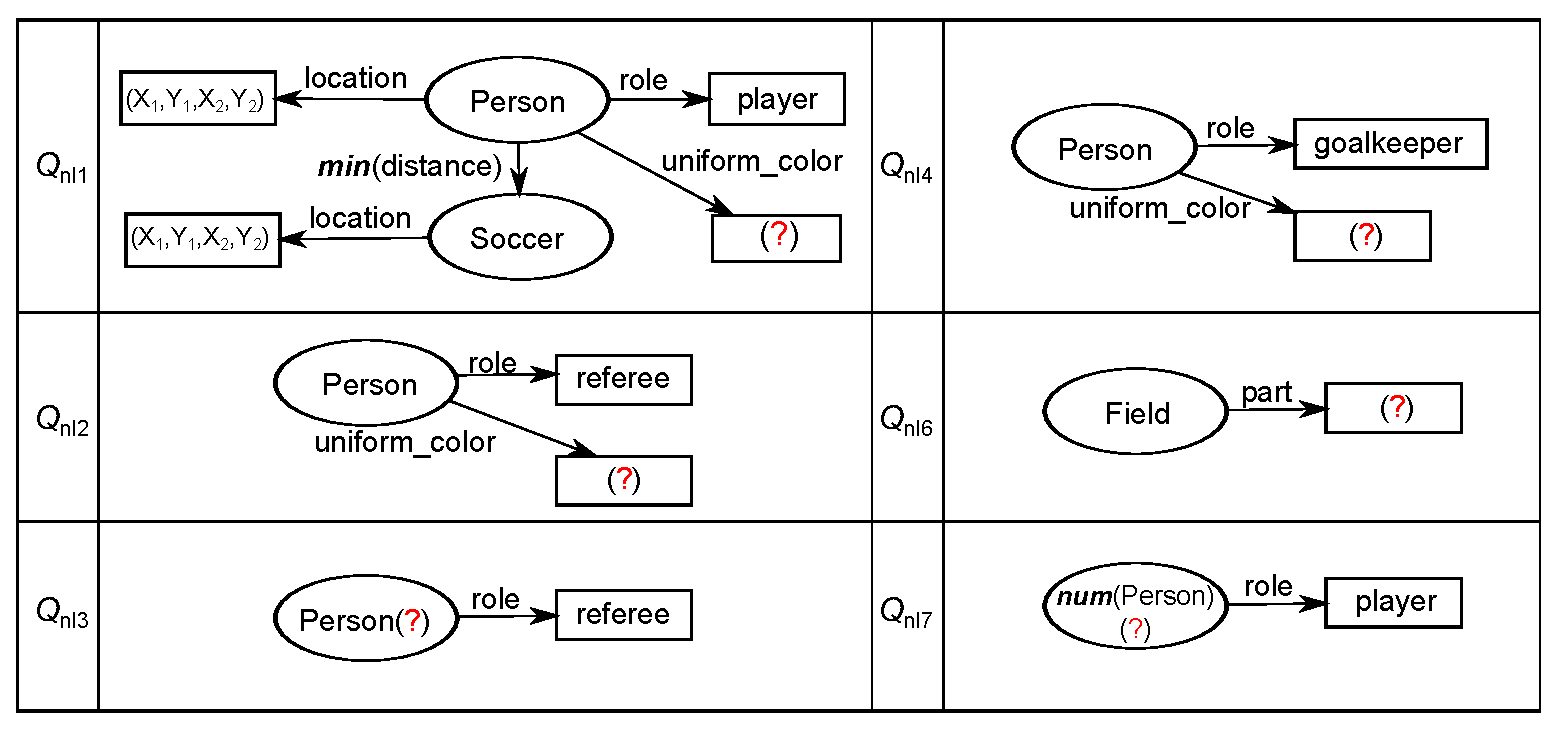
\includegraphics[width=\columnwidth]{queries.eps}
%\caption{Query graphs}
%\label{fig:queries}
%\end{figure}